% Selected DSN2027 manuscript; evidence and release provenance are archived separately.
\documentclass[conference,10pt]{IEEEtran}
\usepackage[T1]{fontenc}
\usepackage{cite,amsmath,amssymb,amsthm}
\usepackage{booktabs,array,multirow,graphicx}
\usepackage{url,microtype}
\usepackage[hidelinks]{hyperref}
\newtheorem{definition}{Definition}
\newtheorem{proposition}{Proposition}
\begin{document}
\title{RevTrace: Preserving Valid Progress across Trusted Feedback Revisions}
\author{\IEEEauthorblockN{Anonymous submission}\IEEEauthorblockA{Regular paper}}
\maketitle
\begin{abstract}
Feedback-driven inference can retract timely output whose computation
remains valid. RevTrace coordinates three decisions: complete-input
eligibility, original selection authority, and support for the Consumer's
whole hypothesis. It retains eligible calls without endorsing their
predictions and preserves accepted results across producer failure.
We give sufficient retention conditions and a conditional selected-trace
refinement argument. In a predeclared 24-speaker stratum, computation
retention increases frontier withdrawals from 12 to 17; joint retention
yields zero. In a matched four-speaker native correction study, offered
audio coverage meeting both delivery deadlines rises from 45.2\% to
99.2\% with unchanged selected histories. Whole-run passes increase from
zero with conservative execution to six of eight with RevTrace.
No illegal installation occurs among 3,976 audited
transitions in fault and sustained-state tests; cold recovery and
no-reset quality failures delimit the service claim.
\end{abstract}
\begin{IEEEkeywords}
dependable inference, feedback state, incremental computation, speculative execution, streaming ASR
\end{IEEEkeywords}
\section{Introduction}\label{sec:intro}
A streaming service can meet its delivery deadlines and still erase
usable progress. A correction selected now can become the input to later recognition
\cite{vu2026streamcorrect}. This feedback dependency creates a service
problem beyond first-delivery latency. In an actual streaming run, a
complete two-second audio interval was visible 1.44~s after it became
ready, meeting its two-second display deadline (D2). At 1.54~s, a trusted
update replaced the whole hypothesis with a shorter snapshot despite its
still-valid dependency path. Identical text returned at 3.72~s, meeting
the eight-second certified-delivery deadline (C8). Both first deliveries
were timely, yet the interval disappeared for 2.176~s
(Figure~\ref{fig:continuity_case}). We call this an \emph{avoidable
withdrawal}: an update retracts a delivered whole view that it still
supports. The client loses progress that the revision did not refute.

\begin{figure*}[t]
\centering
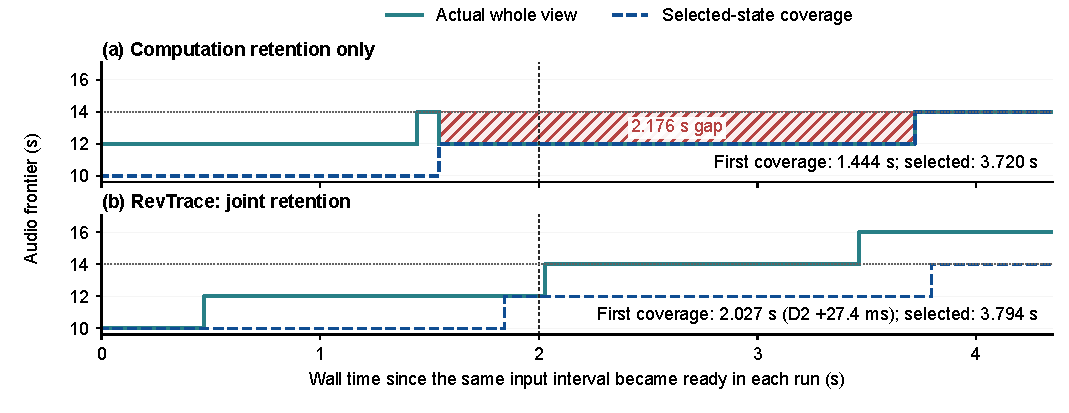
\includegraphics[width=\textwidth]{figures/timely_full_interval_case.pdf}
\caption{On-time delivery does not guarantee continued availability.
Two actual c16-overload runs process the same complete 12--14-s audio
interval using their own ready clocks. (a) Computation-only displays 37
new code points at 1.444~s, withdraws the supported view at 1.544~s and
restores identical text at 3.720~s. (b) RevTrace first displays the same
whole text at 2.027~s, missing D2 by 27.4~ms, and keeps the interval
covered thereafter. Its 3.794-s selected update retains an ahead 16-s view.
The dotted line marks D2 (2~s); both certified deliveries meet C8 (8~s).
These are separate executions with different interleavings, rather than
an event-matched counterfactual.}
\label{fig:continuity_case}
\end{figure*}

The separate RevTrace run in Figure~\ref{fig:continuity_case}(b) first
displays the same whole text slightly after D2, then retains coverage.
Its own next selected update also keeps an ahead view. The trajectories
expose first delivery and continued availability as separate obligations.

A dependable revision service must both reject invalid results and
preserve progress that remains usable. Discarding all older work enforces
a conservative boundary at the cost of service. Preserving computation
alone leaves another gap: the Consumer can still replace its valid ahead
view when a selected state installs. In a predeclared 24-speaker stratum,
computation retention improves timely audio coverage while increasing
backward movements of the displayed audio frontier, or \emph{frontier
withdrawals}, from 12 to 17. Coordinating computation and view retention
yields zero. Valid execution must therefore be connected to continued
availability at the actual Consumer.

One feedback revision can have different consequences for an executing
call, an accepted result, and a displayed hypothesis. RevTrace separates
three judgments. \textbf{[EL] Input eligibility} checks the complete frozen
input and its dependency path under the selected feedback state.
\textbf{[AU] Selection authority} keeps the original selection and ordered
installation bound to the complete original result. \textbf{[SUP] View
support} checks the Consumer's whole hypothesis when that state installs
(Figure~\ref{fig:protocol}). A call's input can be confirmed even when its
own next prediction is wrong. A view can lose support while a future
call's input is unresolved. Producer exit can end new-message authority
while leaving an already accepted result eligible. A birth version,
matching text, or producer-liveness bit cannot stand in for these
different decisions.

Dependency reuse and revocation have established foundations in
incremental dialogue and computation
\cite{schlangen2011incremental,hammer2014adapton,hammer2015names}.
SSBD coordinates draft reuse with display masking~\cite{zeng2026ssbd};
PredGen speculates across evolving speech stages~\cite{li2025predgen}.
RevTrace realizes coordination around a recursively selected feedback
task: complete calls retain the original correction and update, while
the actual whole view is checked independently at selected-state
installation. This provides a concrete use for old work without turning
a prediction into selection authority.

We make three contributions:
\begin{itemize}
\item A service contract exposing avoidable withdrawal and sufficient,
  executable witnesses for complete-call eligibility and whole-view
  support across trusted revisions
  (Sections~\ref{sec:contract}--\ref{sec:continuation}).
\item A joint coordinator that preserves the original selected transition
  relation while retaining eligible calls and supported whole views.
  Its conditional selected-trace argument connects early execution,
  durable selection and supported process failures
  (Sections~\ref{sec:continuation}--\ref{sec:protocol}).
\item Evidence that computation-only retention can worsen visible
  progress, and that confirmed full calls improve timely original-task
  service. Factorial, native and fault controls distinguish these benefits
  from text accuracy, recovery latency and load boundaries
  (Section~\ref{sec:eval}).
\end{itemize}

In the matched four-speaker native study, audio coverage meeting both
deadlines increases from 45.2\% with conservative execution to 99.2\% with
RevTrace; whole-run passes rise from zero to six of eight. A whole-run
pass meets both P99 delivery targets. The independent factorial study explains why
retaining work and retaining its delivered view are separate obligations.

\section{System and Feedback Contract}\label{sec:contract}
\subsection{System and Failure Model}\label{subsec:failure_model}
Each session has an Owner serializing selected transitions, workers
executing frozen calls, and an actual Consumer applying selected facts
and complete provisional hypotheses. Durable storage records the
selected prefix. A Supervisor monitors the processes and preserves the
accepted-input ledger.

We assume one trusted Owner per session, protected selection, immutable
audio and model configuration, unambiguous encoding, collision-resistant
digests, and storage honoring successful synchronization. Used calls must
faithfully consume their frozen inputs. Host receipts bind API objects,
not GPU arithmetic; independent Private and Authority floating-point
executions need not agree.

The interface checks identity, completeness, derived state, and ancestry.
Native resilience supports worker or Owner-group fail-stop on an intact
filesystem; Supervisor, accepted-input ledger, actual Consumer, power
observer, and synchronized storage survive. Their original input clocks
continue through restart. Supervisor/Consumer failure, host power loss,
compromised Owner or Authority, Byzantine code, persistent corruption,
and lost storage are excluded. Controlled wrong-input injections in
Section~\ref{sec:eval} intentionally violate normal Private input fidelity;
we use them to study containment and executor release, not as examples
covered by the lawful-continuation proposition.

\subsection{Feedback creates an execution dependency}
An immutable audio stream supplies a protected selection path producing
\emph{Canonical} facts and a faster \emph{Private} path computing and
displaying provisional hypotheses. Selection can change the next call's
input: StreamCorrect feeds its chosen correction into subsequent
ASR~\cite{vu2026streamcorrect}. We coordinate this dependency as the paths
advance asynchronously.

For a fixed session and execution contract, write an installed fact as
\begin{equation}
 C=(v,F,Z_C,P_C,T_C).
 \label{eq:canonical}
\end{equation}
Here $v$ is the version, $F$ the certified processing frontier, $Z_C$ the
complete selected output, $P_C$ the feedback state, and $T_C$ its bound
text. The contract fixes the model, adapter, decoding, audio identity,
and transformations to $P$ and $T$. Consumer coverage follows the adapter's
publication policy; advancing $F$ need not add characters. Certification
means acceptance by protected selection and installation, separately
from human-transcription accuracy.

The adapter declares a conservative representation of \emph{all mutable
cross-call state that can affect later model inputs, selection, or feedback}.
Telemetry and resources are separate. Qwen passes prompt tokens without
cross-call numerical KV caches. The native adapter additionally carries
audio buffers, token groups, context, alignment position, and decoder
configuration. Comparisons require the same contract: text equality
cannot replace an omitted cursor or numerical cache. The representation
may conservatively include fields unnecessary to a particular call.

\begin{figure*}[t]
\centering
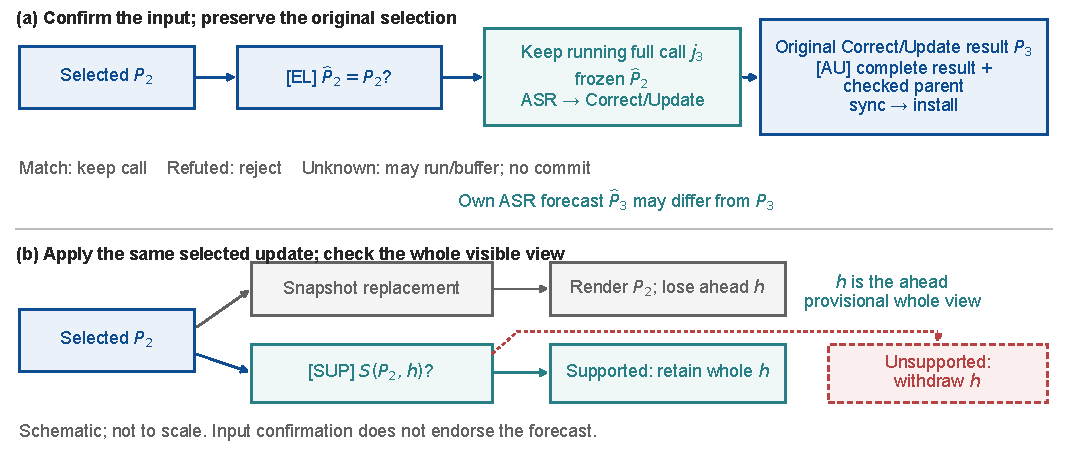
\includegraphics[width=\textwidth]{figures/coordination_protocol.pdf}
\caption{One trusted revision requires separate decisions about work and
its use. [EL] confirms the complete frozen input of $j_3$ against actual
selected $P_2$. [AU] retains original Correct/Update before durable
selection; the call's own prediction can differ from its result.
[SUP] independently retains the whole supported view when $P_2$ installs.
Unknown input remains unresolved while owned calls may run or buffer;
it grants no commit authority. Arrows show decisions and their outcomes;
the dashed red branch marks failed support. This is a causal schematic
without a measured time scale.}
\label{fig:protocol}
\end{figure*}

\subsection{Calls, views and outstanding input}
A complete provisional node $n$ records a frozen call
\begin{equation}
 q_n=(a_n,P_n^-,b_n,\chi_n),\quad
 n=(q_n,Z_n,P_n^+,T_n),
 \label{eq:node}
\end{equation}
where $a_n$ is the input-state frontier, $b_n>a_n$ the audio target, and
$\chi_n$ binds remaining inputs and execution identity. The model may read
the prefix through $b_n$; $a_n$ does not assert token-to-audio alignment.
The adapter derives $P_n^+$ and $T_n$ from a complete result. An in-flight
call has only its frozen input; partial or cancelled tokens supply no node.

The \emph{dependency lifetime} determines usability under the current
root; the \emph{visible lifetime} determines whole-hypothesis retention;
the \emph{physical lifetime} ends only when execution finishes or drains.
A new root can change the first two before the third ends. Their decisions
therefore require separate evidence.

The service retains every accepted input obligation until certified
processing covers it. Discarding a branch, requesting cancellation, or
recovering an old view does not remove that obligation or reset its arrival
clock. In exact mode, a missed deadline never authorizes an uncertified
Canonical transition.

\section{Coordinating Calls and Whole Views}\label{sec:continuation}
\subsection{One revision, three different decisions}
Figure~\ref{fig:protocol} follows a complete call $j_3$. Recognition in
its parent produces a provisional state $\widehat P_2$ while original
Correct/Update is still selecting $P_2$. RevTrace can start $j_3$ on
$\widehat P_2$. When actual $P_2$ arrives at the same frontier, equality
of the entire frozen input confirms $j_3$ under [EL]. Its execution
continues with the same identity. Subscripts identify successive states,
rather than audio seconds; audio, target, EOS, model and decoding bindings
are also fixed.

The call can expose its own prediction $\widehat P_3$, yet original
Correct/Update may choose a different $P_3$. [AU] permits selection of
that complete original result once its parent is installed; it does not
certify $\widehat P_3$. Independently, installing $P_2$ triggers [SUP]
on the actual whole view $h$. A complete path from $P_2$ to $h$ permits
retention; otherwise the Consumer displays the installed state. Losing
this path does not refute the unknown input of a later call. The protocol
therefore distinguishes continuing computation, buffering a result,
selecting a transition and retaining a view.

The following sufficient witnesses formalize these decisions. Producer
failure changes message admission separately, as described in
Section~\ref{subsec:native_resilience}.

\subsection{Complete dependency witnesses}
The central question is whether an old call still belongs to a valid
provisional continuation after trusted feedback advances. Its birth version
records dispatch history. The dependency witness establishes whether it
remains usable now.

Let $x=(F,P_C)$. A complete recorded node provides an edge
\begin{equation}
 (F,P_C)\xrightarrow{n}(b_n,P_n^+)
 \quad\text{if}\quad a_n=F\ \land\ P_n^-=P_C,
 \label{eq:edge}
\end{equation}
under the input, identity, and execution contract of
Section~\ref{sec:contract}. A finite sequence of such edges is a
\emph{valid provisional continuation} of $C$ when each successor consumes
the preceding complete output state at its actual frontier. Write
$C\leadsto n$ for a complete path to $n$. A frozen in-flight successor can
belong to the same continuation, but contributes no usable result until
completion.

\begin{proposition}[Sufficient re-rooting witness]
\label{prop:rebase}
Suppose an old branch contains a complete boundary node at the new certified
frontier $F$, with output state $P_C$. If its subsequent recorded calls form
an unbroken input--output path to the actual branch tip, those nodes are a
valid provisional continuation of $C$. An in-flight successor may continue
when its unchanged frozen input is that tip and its target exceeds $F$.
\end{proposition}
\begin{proof}
The boundary equals $(F,P_C)$, so the first successor satisfies
Eq.~\eqref{eq:edge}. Each subsequent call consumes the preceding complete
output at its recorded frontier under the same contract. Induction reaches
the tip and the unchanged input of its in-flight successor, which supplies
no output yet.
\end{proof}

This establishes dependency validity, not Canonical write authority.
Provisional results remain revisable. The witness follows actual calls
without assuming bitwise equality of different floating-point executions.

A branch born under $v$ can reach $(F,P_C)$ when $v+1$ installs, making
version-only rejection wasteful. Conversely, equal text can hide different
tokens or alignment state; equal state at a different frontier also fails
Eq.~\eqref{eq:edge}.

\subsection{[EL] Retaining computation: \texorpdfstring{$R$}{R}}
The core Qwen guard conservatively implements Proposition~\ref{prop:rebase}.
On installation, it requires a complete Private node at exactly $F$ with
full feedback tokens $P_C$, then checks frozen inputs and frontiers along
complete successors to the actual tip. An intermediate match is insufficient.
An in-flight successor must be the unique tracked task, consume that tip,
and target audio beyond $F$.

Success retains the branch without changing job IDs, birth versions,
inputs, or results; otherwise the Owner fences it and rebuilds from an
allowed state. Boundary-node and unique-slot requirements restrict this
sufficient guard, not every valid reuse scheme.

\subsection{[SUP] Retaining an actual view: \texorpdfstring{$S$}{S}}
A snapshot Consumer can replace a valid ahead view with a shorter
certified snapshot despite computation retention. RevTrace maintains
separate certified and provisional whole-hypothesis lanes, without an
uncertified suffix splice or certified-prefix status for retained views.

For a Canonical application, $S$ checks the complete visible node's input
directly against $(F,P_C)$ or follows complete published ancestors to
that boundary. Missing, cyclic, or ambiguous ancestry is rejected. Unlike
$R$'s conservative guard, a directly rooted published call needs no extra
Private boundary node.

Before actual application and its receipt, the kernel checks the preview
against the durable root, registered results, dependency path, and bound
text/frontier. A caller-supplied compatibility flag cannot replace these
records.

\begin{proposition}[Continuity at a compatible application]
\label{prop:continuity}
Immediately before an authorized Canonical application, let the visible
whole provisional view $h$ be ahead of its new frontier $F$. If $S$ proves
$C\leadsto h$ and no independent withdrawal mode is invoked, that
application advances the certified lane and preserves $h$ unchanged.
\end{proposition}
\begin{proof}
The authorized compatible-and-ahead branch installs $C$ in the certified
lane while retaining $h$'s node, text, and frontier. That application
therefore withdraws none of $h$.
\end{proof}

Incompatible updates must withdraw the view, and later valid results can
revise it. This is a per-application property, not global monotonicity.
Snapshot consumption and conservative recomputation can be safe; the
four-arm study measures the extra progress and cost of joint retention.

\subsection{Native feedback and conditional full calls}
\label{subsec:native_full_calls}
StreamCorrect supplies a concrete recursive feedback task
\cite{vu2026streamcorrect}. For complete closed state $P$ and accepted
audio $X$, expose its recognition boundary as
\begin{equation}
 A(P,X)=(B,M),
\end{equation}
where $B$ contains ordered beam candidates and $M$ the engine state and
inputs needed by original Correct/Update. Candidate order,
prompts, returned token IDs, selection, and update rules remain intact.

Before learned correction finishes, the original update tail with a typed
first-beam identity prediction produces provisional closed state
$\widehat P^+$. It is a dependency projection, not a complete selected
result. A second worker can run the next \emph{complete original call} on
that conditional input; both GPUs host the full recognizer--corrector.
Its own prediction may be wrong even when its input later matches.
Original Correct/Update determines the complete result.

When the parent installs, the Owner compares the call's complete frozen
start state, actual frontier, contract, and session epoch with it. Equality
confirms the unchanged owned call: it continues if running, or becomes
eligible for ordered selection if complete. Job ID, birth, producer
incarnation, inputs, and execution history stay unchanged.

An earlier ancestor mismatch can remove current view support without
refuting a later complete input. Cancellation before correction requires
a disagreeing actual selected state at that call's own start frontier,
coverage of its target without remaining use, or a changed epoch. An
unresolved future parent supplies none of these proofs. The view can
therefore require withdrawal while the call remains unresolved.

This native input witness and the core Qwen boundary-node/unique-successor
guard are different sufficient implementations of the continuation
relation. Neither grants write authority. Both use a whole-view Consumer
that keeps certified and provisional provenance separate. The native
comparison holds two complete workers fixed and varies conditional
dispatch and retention; ready-only ASR handoff is a separate developmental
control.

For a call $j$, its complete frozen input is \emph{confirmed} when it
matches the installed parent, \emph{refuted} when an actual selected state
at its start frontier differs, and \emph{unknown} without either witness.
Covered targets and fenced sessions cannot supply selected results.
Table~\ref{tab:coordinator} separates these input decisions from actual
view application.

\begin{table}[t]
\centering
\caption{Event-driven coordination of confirmed calls and supported
whole views.}
\label{tab:coordinator}
\begingroup\small
\setlength{\tabcolsep}{3pt}
\begin{tabular}{@{}>{\raggedright\arraybackslash}p{0.17\columnwidth}>{\raggedright\arraybackslash}p{0.32\columnwidth}>{\raggedright\arraybackslash}p{0.46\columnwidth}@{}}
\toprule
Event & Required evidence & Action\\
\midrule
Dispatch & Ready worker; accepted audio and an eligible session start &
Use the unchanged dispatcher; freeze the full input, target and original
job identity.\\
ASR result & Bound recognition result and contiguous provisional path &
Extend the typed prediction and publish its provisional view; do not
select it.\\
Full result & Bound original result [AU]; complete input status [EL] &
Select if confirmed, buffer if unknown; deny use if refuted, covered or
fenced.\\
Select ready & Confirmed complete result and unchanged installed parent &
Synchronize the bound fact before installation; record the selected state
and recheck pending calls.\\
Consumer update & Ordered fact, actual parent and whole-view support [SUP]
$S(C,h)$ & Advance the certified view. Retain the complete ahead $h$ when
supported; otherwise render the installed state.\\
\bottomrule
\end{tabular}
\endgroup
\end{table}

The dispatcher scans available workers and sessions in their existing
order. Within each session it tries missing selected work before a
conditional tail, subject to the ahead bound; it imposes no global
selected-work priority across sessions. Unknown input grants neither
selection nor a refutation-based cancellation proof. Replacing a typed
prediction with its complete result keeps only the suffix that consumes
the actual output contiguously. Physical release and producer-failure
handling follow Section~\ref{sec:protocol}.

% Integrated method extension; formal paired evaluation remains separate.
% Source audit: resilience_policy._commit; FactStore.commit/_replay;
% SurvivorConsumer._fact/replay_fact. No whole Python/CUDA proof is claimed.
\subsection{[AU] Preserving the selected program}
\label{subsec:native_refinement}
Let $P \mathrel{\Rightarrow_{\mathcal A,X}} P'$ denote a transition allowed
by the original protected program on accepted immutable input $X$.
The relation may be nondeterministic. A complete original call includes
its original selection and update, or its declared buffer-only path;
a typed identity projection is not such a result. We project a protocol
execution onto its distinct durable selected facts, deleting speculation,
waiting, local rejection, cancellation, collection, and repeated delivery.
This restricted projection follows the standard stuttering view of
refinement~\cite{abadi1991refinement}; provisional whole-view behavior
remains outside its alphabet and has a separate compatibility property.

\begin{proposition}[Selected-trace refinement]
\label{prop:refinement}
Assume sufficient declared state, faithful execution of frozen inputs,
exclusive serial selection, correctly bound message identities, and
storage that honors successful synchronization. If each new durable fact
binds a complete original call whose full input equals the preceding
selected cut, retains the call's original identity, was admitted under
valid message authority, and is synchronized before installation or certified
application, then the projected facts form an execution allowed by
$\mathcal A$. Replaying an existing fact adds no transition.
\end{proposition}
\begin{proof}
The initial cut belongs to $\mathcal A$. Deleted actions do not extend
the prefix. Each new fact binds a complete original call on exactly the
preceding cut and accepted input, hence an allowed next edge regardless
of dispatch time. Synchronization precedes privileged application.
Recovery replays the same checked identities, including a fact first
consumed after an Owner crash, without adding an edge. Induction proves
the claim.
\end{proof}

The durable append is the selection boundary; installation and consumption
do not select again. Already accepted buffers retain their producer
identities after exit, whereas new fenced messages are inadmissible.
The certified frontier derives only from checked facts; ahead views remain
provisional. Input confirmation does not certify predicted next states.

A separately frozen specification explores 6,231 two-frontier normal
states and 14,074 one-frontier failure states, each to a 12-event depth,
with 27 named controls. An independent trace checker binds actual facts
and whole-view applications to original call receipts. The specification
is not extracted from the runtime; depth bounds truncate exploration,
and neither check verifies all Python, CUDA, or operating-system behavior.
Exact equality with a fixed neural reference is separate empirical evidence,
rather than a premise that arbitrary GPU reruns must be bitwise identical.


\section{Execution Protocol}\label{sec:protocol}
\subsection{Complete results and physical ownership}
In the core runtime, dispatch binds session,
incarnation, job, input, target, and contract. A row returns either a
complete result with re-derived state/text or cancellation without partial
state. Complete rows can be installed and consumed before their batch
finishes. Only all terminal rows and device synchronization authorize
\texttt{BatchDrained} and executor reuse. The native process lifecycle
below has separate evidence.

\subsection{Covered work and safe-point exit: \texorpdfstring{$K$}{K}}
For the tested use model, $K$ requests exit when the installed Canonical
frontier covers a proposal's target and it has no remaining declared use.
This differs from $R$: valid work beyond the new root can remain useful.
Workers observe \texttt{CancelRequest} at decode boundaries; completion
can win, but each row has one terminal outcome. Static batches are not
compacted or refilled; masked costs and drain delays remain measured.

\subsection{Durable facts and outstanding input}
Before acknowledgment, synchronized frames bind parent/next states,
request identity, selected complete result, and receipt; recorded deltas
must reconstruct the state. Group-ready commit shares synchronization
among validated sessions without a collection timeout or cross-session
atomic transaction. Uncertain append/application outcomes block writes.
Write-ahead recovery~\cite{mohan1992aries} reconstructs facts and identities;
the native extension binds this to original correction calls.

\subsection{Validation boundaries}
Propositions~\ref{prop:rebase} and~\ref{prop:continuity} concern the stated
guards and compatible applications. The artifact retains an earlier,
separately frozen recovery prototype and its bounded model and crash
results; they do not validate the later core or native fault paths.
The selected-trace argument of Proposition~\ref{prop:refinement}, its
finite specification, and actual execution checks have distinct scopes.

\subsection{Continuing through delivery and process failures}
\label{subsec:native_resilience}
Each job has an Owner namespace and monotonic issue number; each physical
slot has a worker incarnation, using established RPC identity principles
\cite{birrell1984rpc}. Fencing removes future message authority without
renaming already accepted complete results.

\paragraph{Local rejection and physical release}
The ingress guard rejects exact duplicates and fenced messages locally;
they cannot mutate selected state or release newer leases. Contradictory
currently owned contents freeze writes. Per-incarnation Pipes and receiver
threads isolate incomplete frames. Replacement requires process exit,
CUDA release and joined receivers. Strictly validate complete receipts
from the sealed channel before fencing the incarnation and retiring
unfinished work. Accepted buffers and supported views retain their
original identities.

\paragraph{Durable selection and recovery}
A synchronous hook binds complete parent/next states, original correction
and IDs, job, Owner/session epochs, and producer incarnation. Framing,
checksums and chaining protect the fact; synchronization precedes
installation/publication. Uncertain writes freeze the writer. Recovery
discards only an incomplete final frame; complete corruption fails.
These conventional write-ahead rules~\cite{mohan1992aries} bind the
original feedback transition.

The surviving Supervisor preserves the input ledger and original clocks.
After old physical ownership ends, it advances the Owner namespace,
replays the verified fact prefix, and cold-starts workers. Replay adds no
inference; old publications gain no new authority. Both policies share
this coordinator, durability, recovery, and actual Consumer.

\paragraph{Conditional continued service}
\phantomsection\label{prop:continued_service}
For finite accepted work after finite supported failures, further progress
requires readable storage, eventual physical release/loading, terminating
original calls that advance frontiers, fair Owner/Consumer scheduling,
and sufficient service budgets. This is not an RTO or D2/C8 guarantee;
loading, replay and recomputation retain their original clocks.

\paragraph{Control history}
Roots, calls, buffers, visible views and outboxes pin their dependencies.
Actual acknowledgment releases publication references, while the visible
view stays pinned. Namespace/issue high watermarks prevent reuse after
collection. Unreferenced terminal and audit windows have fixed limits;
diagnostics stream to disk. These bound protocol entries relative to live
dependencies, separately from current state, cumulative text and total
memory.

\section{Evaluation}\label{sec:eval}
\subsection{Design, comparators and service endpoints}
We evaluate whether [EL], [AU] and [SUP] jointly preserve legal progress
under unchanged selected feedback histories. Core factorial controls
separate computation retention from whole-view retention; native tests
measure confirmed full calls executing the original correction task.
An instrumented FIFO Consumer records actual applications. All accepted
inputs keep their original ready times through cancellation and recovery.

\paragraph{Core implementation and sources}
Two 24-GB RTX~3090s host an FP16 Private worker and FP32 Authority worker.
Qwen3-ASR~1.7B~\cite{shi2026qwen3asr} is primary; Whisper base.en
\cite{radford2023whisper} tests a second state adapter. Complete-row
delivery, at most 16 rows per batch, a 256-token limit, the protocol kernel
and synchronized journals are shared. Physical early exit is disabled
in this factorial study, separating retention from cancellation.
Initial loading precedes the service clock. Energy integrates both
physical boards over the declared service window.

Independent confirmation uses 24 previously unused LibriSpeech speakers
\cite{panayotov2015librispeech}, metadata-selected before inference and
partitioned into three eight-speaker cohorts, totaling 714.110~s per arm.
Its 110 cells comprise 60 primary cells (three cohorts, two backends, two
arrival patterns, five arms), 20 fresh-process repeats on cohort~A and 30
coarser-feedback controls. At $\rho=1$, Authority advances every 2~s;
$\rho=3$ changes selection frequency and feedback segmentation. Arrivals
are simultaneous or staggered by 0.25~s. Repetitions and arms reuse these
sources; speakers are the independent acoustic units.

\paragraph{Named comparisons}
\emph{Checked snapshot + recomputation} ($R_0S_0$), \emph{View retention
only} ($R_0S_1$), \emph{Computation retention only} ($R_1S_0$), and
\emph{RevTrace: joint retention} ($R_1S_1$) share validation, durability,
input accounting and physical execution. Disabling $R$ rebuilds work
from selected feedback; disabling $S$ replaces the provisional view
with the installed snapshot while retaining the same dependency checks.
The \emph{Alternative joint implementation} is our complete positive
control: another policy instantiation of the same retention and Consumer
conditions on the shared execution/commit substrate. External prior work
and our author-built comparators have separate identities.

\paragraph{Endpoints}
For offered interval $i$, $w_i$ is audio duration, $r_i$ its original
ready time, $d_i$ first actual visible coverage and $c_i$ first actual
certified coverage. Audio coverage meeting both deadlines is
\begin{equation}
 A_{2,8}=\sum_i w_i\,\mathbf{1}
 \{d_i-r_i\leq2\ \land\ c_i-r_i\leq8\}.
 \label{eq:credit}
\end{equation}
All offered intervals, including partial end-of-stream (EOS) tails,
remain in the denominator. Whole-run passes require display P99 at most
2~s (D2) and certified-view P99 at most 8~s (C8), over offered frontiers.
P99 weights frontier observations; $A_{2,8}$ weights duration, so a P99
pass may coexist with a small uncredited tail.

We separately count visible-frontier withdrawals, erased code points and
deficit below the previously observed frontier. Retrospective whole-text
support compares a first actual view with later selected text at that
view's own frontier. This is distinct from dependency validity [SUP],
human word/character error rate, and new character count. Independent
checks reconstruct complete selected $F/Z/P/\mathrm{text}$ histories and
actual consumed input paths from original outputs.

\subsection{Does retaining computation retain delivered service?}
Retaining computation alone can improve timeliness while increasing
withdrawal. Figure~\ref{fig:main_evidence}(a) shows the predeclared Qwen,
$\rho=1$, staggered stratum. With the same selected histories, computation
retention raises covered audio from 654.115 to 664.150~s but withdrawals
from 12 to 17. View retention alone reduces withdrawals to 1 but covers
628.435~s. RevTrace jointly covers 680.760~s with zero frontier withdrawals:
26.645~s above recomputation and 16.610~s above computation-only.

\begin{figure*}[t]
\centering
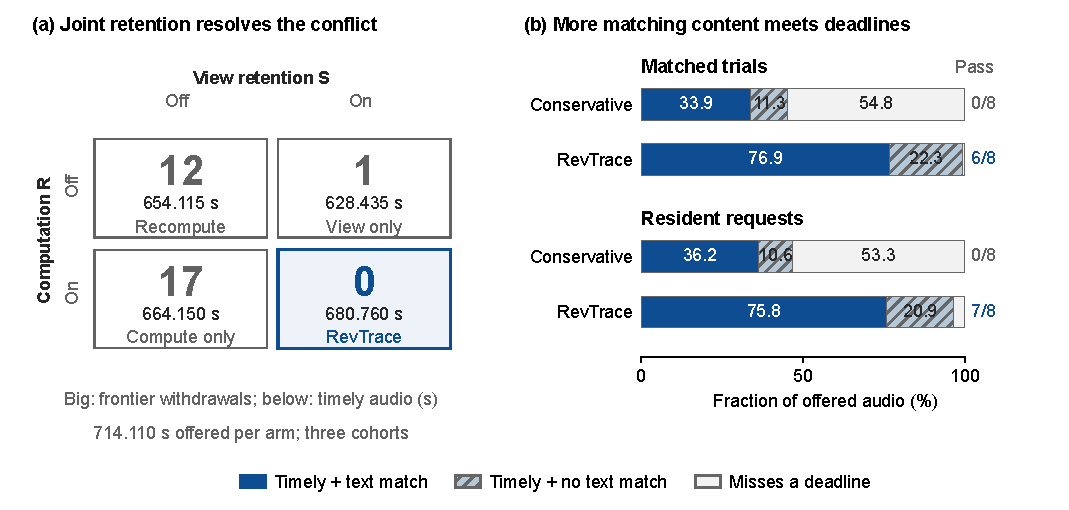
\includegraphics[width=\textwidth]{figures/joint_and_content.pdf}
\caption{Retained work and retained service require coordinated decisions.
(a) The predeclared 24-speaker stratum: each cell sums three eight-speaker cohorts'
frontier withdrawals and audio coverage meeting display 2~s/certified 8~s
deadlines over 714.110~s per arm. The four matrix arms and our separate
Alternative joint positive control (15 runs total)
fail whole-run D2. (b) Final native matched and resident banks each offer
66.340~s per policy on four existing sources. Stacks separate timely
same-frontier whole-text agreement, other timely coverage and uncovered
audio; text agreement is retrospective against selected model output.
Unlabelled tails are the remainder to 100\%, with rounded labels.
Passes count matched trials or resident requests meeting display P99
$\leq2$~s and certified P99 $\leq8$~s.}
\label{fig:main_evidence}
\end{figure*}

Cohort-wise credit interaction,
$I=Y_{11}-Y_{10}-Y_{01}+Y_{00}$, is $+18.530$, $+6.205$, and $+17.555$~s.
These are three queue-coupled cohort contrasts, not independent deadline
windows. RevTrace's text remains revisable: 569 characters are erased
despite zero frontier withdrawal. Median per-run display P99 is 2.329~s,
above D2, so the benefit is retained progress under overload rather than
a whole-run service pass.

The Alternative joint implementation also yields zero withdrawals and 569
erased characters, with 667.530~s coverage and 2.534-s median P99. It
reproduces the supported-view behavior on the common substrate. Across
confirmation, 144 matched history groups and 22 positive-control pairs
agree on complete selected histories. Thus the comparison holds the
feedback task fixed while changing how valid work becomes service.
\par\noindent\textbf{Finding 1: retained computation does not ensure retained service.}
[EL] can retain work whose presentation a snapshot Consumer still removes.
Joint [EL]/[SUP] coordination preserves the supported ahead view.

\subsection{Timely native service with original full calls}
\label{subsec:native_retention_eval}
Input-confirmed full calls improve timely service while preserving the
original feedback task. In the final four-speaker comparison, RevTrace
raises audio coverage meeting both deadlines from 45.2\% to 99.2\% and
whole-run passes from zero to six of eight
(Table~\ref{tab:native_full_confirm}). The StreamCorrect adaptation retains
original learned correction and feedback, using fixed 500-ms inputs,
no VAD, and FP32 execution~\cite{vu2026streamcorrect}. Both author-built
policies have two complete workers, the same ASR early-view Consumer and
neural warmup. Conservative execution waits for selected parent feedback;
RevTrace starts conditional full calls and retains them when their
complete inputs are confirmed.

\begin{table}[t]
\centering
\caption{Final native RevTrace improves timely coverage with the original
selected task. Each policy offers 66.340~audio-s over four previously
measured speakers and two fresh trials per speaker. Coverage and both-board
energy are totals; D99 is the median of per-run display P99. Energy spans
the common external origin-to-confirmed-physical-model-drain window.
Pass counts trials meeting both whole-run D2/C8 criteria.}
\label{tab:native_full_confirm}
\small\setlength{\tabcolsep}{3pt}
\begin{tabular}{@{}lrrrr@{}}
\toprule
Policy & \shortstack{Timely\\coverage (s)} & \shortstack{D99\\(s)} &
\shortstack{Energy\\(kJ)} & Pass\\
\midrule
Conservative & 30.000 & 4.759 & 47.019 & 0/8\\
RevTrace & 65.822 & 1.638 & 43.952 & 6/8\\
\bottomrule
\end{tabular}
\end{table}

\paragraph{Task fidelity and matched sources}
The matched version study holds four AISHELL-1 sources
\cite{bu2017aishell}, models, warmup, allocator and GPU-role rotation fixed:
two versions, two policies and two fresh repeats give 32 runs. All 544
selected transitions match complete original inputs/outputs, correction
and returned IDs under the declared static code-version mapping. The
sources were initially selected by metadata in an 8--9-s band after
freezing the earlier prototype. Its separate 16-run independent bank
matched all 272 original transitions, with five character edits over 81
unique reference characters (6.17\% CER) in both arms. The matched study
reuses those speakers; repetitions do not add independent acoustic units.
Every original 500-ms frontier and partial EOS remains in the accounting.

\paragraph{Reliability-extension cost and EOS margin}
Final RevTrace uses 6.52\% less common-window board energy than final
Conservative. Relative to the earlier matched RevTrace prototype, energy
increases by 10.61\% (39.735 to 43.952~kJ). That prototype achieves 8/8
passes and 66.340~s of coverage in the matched study; its earlier
independent bank separately improves coverage from 37.0 to 66.33975~s
and passes from 0/8 to 8/8.
Final RevTrace's two remaining failures are S0908 EOS intervals, whose
display P99 increases by 0.163/0.050~s against the earlier matched version.
Other paired timing differences have both signs. The common model-drain
window supports this energy comparison; source-specific cleanup and
certified-EOS windows remain separate endpoints.

\paragraph{Resident independent requests}
RevTrace raises joint D2/C8 passes from 0/8 to 7/8 requests, and timely
coverage from 31.0 to 64.118875 of 66.33975~s. Models load once per trial;
both worker PIDs persist across four pre-registered independent requests.
The next request starts only after actual certified consumption of the
previous file EOS. Two policies and two fresh trials preserve all 272
original transitions and each request's own input clock. The second
S0908 repeat has D99 2.229~s. This single-outstanding closed-loop contract
tests residency, rather than online VAD or open-arrival capacity.

\paragraph{The same content arrives earlier}
Figure~\ref{fig:main_evidence}(b) separates deadline coverage from content
support. Timely coverage whose whole first view retrospectively matches selected
text at that view's own frontier $G$ rises from 22.5 to 51.0~s in matched
runs and from 24.0 to 50.259~s in resident requests. RevTrace's remaining
14.822/13.860~s of timely coverage does not match; unknown coverage is zero.
Raw and whitespace comparisons agree. Each policy in either bank
introduces 180 code-point occurrences, retracts 14 and leaves 166
last-visible. All-offered whole-text matches are 106/136 for Conservative
and 104/136 for RevTrace. The gain is earlier delivery of matching content,
with unchanged character counts; this comparison with selected model
output is distinct from human-transcription accuracy.

\paragraph{Input confirmation and view retention}
The earlier independent bank has 92 promoted calls whose recognition
begins before selected parent completion; 20 have wrong own predicted
ends. Twenty-four invalid/covered calls stop after ASR and two complete
wrong-input results are discarded. These observations separate input
eligibility from prediction correctness.

The final matched bank has no compatible-ahead application and therefore
does not repeat the core factorial continuity test. Resident RevTrace has
one nonempty opportunity: a 5.0-s whole view survives a compatible 4.5-s
selected update with the same tip and job. Its 0.817-s Consumer event-state
holding interval spans that update and ends at legitimate supersession.
Each RevTrace bank also contains two necessary incompatible withdrawals;
final objects are right-censored at the last actual same-source observation.
\par\noindent\textbf{Finding 2: confirmed inputs accelerate the original task.}
Original selection [AU] remains intact when [EL] confirms early full calls;
whole-view retention still requires [SUP] independently.

\subsection{When does the opportunity appear or disappear?}
The opportunity is a supported whole view ahead of a newly installed
selected frontier. In the headline RevTrace arm, 18 of 368 updates encounter
and retain one; computation-only encounters 17 and clears all 17. Under
synchronized arrivals, RevTrace encounters only 3 of 368 and covers 0.790~s
less than computation-only. A fresh staggered repeat on cohort~A also
changes the timing ranking: 226.320 versus 230.565~s, $I=-2.245$~s.
Compatible relative progress determines the benefit; the three positive
primary contrasts do not establish an invariant speed advantage.

\begin{table}[t]
\centering
\caption{Operating boundaries remain visible. Each workload has four
arms and three fresh processes (48 runs total). Pass counts cover all 12
runs; D99 ranges span three RevTrace observations, and timely-loss windows
list computation-only/RevTrace counts. Source mix expands with sessions. Full 48-point
plots and all endpoints remain in the artifact.}
\label{tab:operating_workloads}
\small\setlength{\tabcolsep}{3pt}
\begin{tabular}{@{}lccc@{}}
\toprule
Workload & D2/C8 pass & \shortstack{RevTrace\\D99 (s)} &
\shortstack{Timely-loss\\windows}\\
\midrule
8 sync &12/12 &1.426--1.528 &1,0,0 /0,0,0\\
8 staggered &12/12 &1.704--1.955 &1,2,1 /0,0,0\\
12 staggered &0/12 &2.197--2.299 &1,1,3 /0,0,0\\
16 staggered &0/12 &2.801--3.223 &10,12,9 /0,0,0\\
\bottomrule
\end{tabular}
\end{table}

Table~\ref{tab:operating_workloads} summarizes 36 predeclared development
runs (8 synchronized, 8 staggered, 16 staggered sessions) and 12 exploratory
midpoint runs (12 staggered). Each arm offers 121.205/185.300/250.180~s
at 8/12/16 sessions. These are explicit workloads with different source
mixes. At 8 sessions all arms meet whole-run D2/C8; RevTrace synchronized
display P99 is 1.426--1.528~s and staggered reaches 1.955~s. Two 0.215-s
tails remain uncredited despite their P99 passes. At 12 and 16 sessions
all runs fail D2 and pass C8. At 16, RevTrace's extra coverage over
computation-only is +18.910,+5.055,$-7.225$~s; P99 improves in one repeat.
Its continuity distinction is stable: compatible withdrawals are zero
versus 16/17/12.

A secondary analysis follows intervals already delivered within D2 whose
eventual certified coverage also meets C8. At each selected application,
the complete dependency path classifies compatible loss separately from
necessary revision. Loss ends when actual coverage returns or is
right-censored at the next selected root. Computation-only has 10/12/9
such windows at 16 sessions, with 24.903/23.635/15.736 audio-s$\times$wall-s
deficit; RevTrace has none. Holes intersect the original D2 read point
for 6.000/10.675/4.000~s of distinct audio. The 12-session strong witness
is not established: computation-only's smaller losses never include a
timely complete non-EOS interval under its frozen criterion.
\par\noindent\textbf{Finding 3: continuity and first delivery have different boundaries.}
Retaining a supported view removes an avoidable withdrawal; whether
enough work arrives before D2 remains a separate scheduling and load outcome.

\paragraph{Quality and cost}
Headline Qwen arms share WER 26/1908 (1.36\%) and selected histories.
Retrospective same-frontier whole-text agreement leaves their credits
unchanged. Elsewhere RevTrace's raw comparison removes 2~s in the 16-session third
repeat and 2~s in each midpoint's first two repeats, although the frozen
normalizer agrees. Whisper WER is 83.12\% at $\rho=1$ versus 11.53\% at
$\rho=3$; changing its feedback contract changes quality. Headline board
energy spans 59.16--59.73~J/audio-s across five arm medians. At 16 sessions, RevTrace reduces total
model time by 0.66--1.59~s over recomputation, while wall-time and energy
differences change sign. Retained progress is the measured benefit;
inference cost and overload are independent boundaries.

\subsection{Preserving acquired results through process failures}
\label{subsec:same_source_validation}
The final coordinator preserves acquired results without granting old
messages new authority. Both policies share models, durability, guards,
recovery and Consumer. Initial loading and fixed warmup precede service;
replacement loading, replay, recomputation and physical drain retain the
original clock.

Six conditions, two policies and two fresh processes on one development
clip give 24 short trials, plus four EOS/compatible-view regressions.
Together with eight sustained-state trials below, these 36 trials contain
3,976 durable transitions independently bound to complete original call
receipts and actual Consumer applications, with zero illegal installations
or incorrect owned-message rejections. Eight duplicate/late messages cause
no selected-state mutation; eight worker deaths have confirmed physical
replacements. Conditional calls supply 354 durable facts: 352 have original
Owner installation records, and two first reach the Consumer through
recovery. In four worker-after-ASR cases, a previously consumed whole view
remains across producer exit/fencing until legitimate correction. Its
support, rather than the producer's continued presence, determines retention.

\begin{table*}[t]
\centering
\caption{Fault containment preserves legality; cold recovery still misses
the original service deadlines. The 24 short trials all finish with zero
illegal installations. Each row covers two fresh trials on the same clip;
RevTrace uses input-confirmed full calls. Rejected messages cause zero
selected-state mutations ($\Delta C$). Ranges are observed minima/maxima.
New result measures fault to actual certified consumption of a new fact
whose call completes after the fault, separately from old-fact replay and
replacement readiness. Pass counts joint whole-run D2/C8; EOS counts D2
misses. Both-board energy runs through physical drain.}
\label{tab:native_reliability}
\begingroup\small
\setlength{\tabcolsep}{3pt}
\begin{tabular}{@{}llrrrrr@{}}
\toprule
Condition & Policy & Reject / $\Delta C$ & New result (s) & D2/C8 pass & EOS miss & Energy (J) \\
\midrule
\multirow{2}{*}{No fault} & Conservative & 0 / 0 & -- & 0/2 & 2 & 6566--6574 \\
 & RevTrace & 0 / 0 & -- & 1/2 & 1 & 5896--5911 \\
\multirow{2}{*}{Duplicate / late} & Conservative & 4 / 0 & -- & 0/2 & 2 & 5701--5893 \\
 & RevTrace & 4 / 0 & -- & 1/2 & 1 & 5538--5846 \\
\multirow{2}{*}{Worker after ASR} & Conservative & 0 / 0 & 1.90--2.22 & 0/2 & 2 & 5182--5401 \\
 & RevTrace & 0 / 0 & 2.15--2.21 & 0/2 & 2 & 5447--5647 \\
\multirow{2}{*}{Worker partial frame} & Conservative & 0 / 0 & 2.10--2.25 & 0/2 & 2 & 4775--5178 \\
 & RevTrace & 0 / 0 & 1.76--2.23 & 0/2 & 2 & 5492--5594 \\
\multirow{2}{*}{Owner before durable} & Conservative & 0 / 0 & 86.42--108.08 & 0/2 & 2 & 24549--28019 \\
 & RevTrace & 0 / 0 & 64.61--107.09 & 0/2 & 2 & 19571--26557 \\
\multirow{2}{*}{Owner after durable} & Conservative & 0 / 0 & 83.90--87.05 & 0/2 & 2 & 22415--24200 \\
 & RevTrace & 0 / 0 & 101.80--104.44 & 0/2 & 2 & 26483--27171 \\
\bottomrule
\end{tabular}
% Presentation labels only: Conservative=conservative; RevTrace=fullcall.
% All 24 original short trials completed; independently checked illegal installs=0.
% Range and row values copy frozen FIGURE_TABLE_FORMAL36_v5 / development S0908 only.
% Regression4 and sustained8 retain their separate ALL36_MACHINE_TABLE identities.
% New-result calls may already be in flight on a surviving worker.
% -- is not applicable, not zero; original clocks, failures and energy remain unchanged.

\endgroup
\end{table*}

Worker and Owner failures preserve legality but have different service
costs (Table~\ref{tab:native_reliability}). Normal and duplicate RevTrace
each pass one of two trials; the other misses D2 only at EOS. All
worker-fault trials fail D2 but pass C8; Owner-fault trials fail both.
Old durable facts reappear in 1.36--1.81~s, whereas new certified
post-fault completions take 64.61--108.08~s in Owner cases. A surviving
worker can finish a call before replacement readiness, so replay, new
results and replacement loading have separate recovery clocks.

\paragraph{Complete buffers across producer death}
Two matching and two mismatching timing controls test the accepted-result
case absent from the bank above. A transport fixture holds the parent
after original ASR and the child after sending its complete original
result. After the Owner registers the result, we kill its producer,
verify exit, CUDA release, sealed-channel validation and fencing, then
release original parent correction. Both matching results install and
are consumed once with their original job, birth and incarnation; both
mismatches are rejected against the actual same-frontier parent. Positive
cases also finish a subsequent independent request. These controlled
interleavings establish retention and rejection, rather than fault-time
SLOs. Independent reconstruction corrects an audit-indexing defect over
unchanged traces; the original failed audit gates remain in the artifact.
\par\noindent\textbf{Finding 4: producer failure and result invalidity are different.}
Fencing ends future message authority while eligible, already accepted
results retain their original identities and permitted uses.

\paragraph{Sustained-state stress and its limits}
Two metadata-selected AISHELL-1 speakers contribute 24 utterances each,
concatenated as exact PCM into 228.51025/208.1003125-s streams without join
resets. A continuous original-engine reference and 875 separately restored
steps agree on complete state, correction and IDs, crossing 398/357 buffer
shifts and 353/252 context changes. Eight serving trials produce 3,500
matching selected steps. Unpinned terminal and each audit class stay at
most 64 entries; live dependencies, state/output bytes, Owner RSS and
cumulative logs are separate.

All eight trials fail D2/C8 (display P99 449.727--502.952~s). Both policies
reproduce severe original-task insertion errors: CER 3103/486 (638.48\%)
and 1313/522 (251.53\%). RevTrace uses more energy. The original length
guard can skip decoding, so frontier coverage need not add text. These
are state/collection stress tests rather than deployable continuous ASR.
Across all 36 trials, the checker preserves 90 compatible-ahead
dependency-tip applications and records 1,118 necessary incompatible
withdrawals. Internal tips need not add text; these controlled counts
do not estimate natural prevalence.

An independent dispatch audit finds 360 eventual matches among 1,901
conditional inputs; 1,541 are refuted, none unresolved. Six matched jobs
never become durable after injected failures. Workload-specific ratios
remain separate. Original-clock misses and a conservative offline
excess-length bound precede the after-trim 448-token condition on each
long stream; neither yields online prefix CER or a unique causal diagnosis.

% Compressed earlier K24 support; full measured ledger remains in the artifact.
% This core execution evidence is separate from native failure validation.
\subsection{From physical release to supported service}
\label{subsec:release_evidence}
A separate 24-run core study crosses $R$ and $K$ with $S$ enabled,
two arrival patterns and three fresh processes, using a frozen
wrong-conditioning fixture. Selected histories and WER $14/687$ match;
all 675 same-input/prompt/audio/peer-order pairs return identical outputs.
Synchronized $R1$ releases the next 16-row computation 473--577\,ms
earlier. All 96 following rows are actually consumed and their whole
texts match later same-frontier Canonical text. Only 6/6/1 rows switch
from deadline miss to hit. Adding $K$ changes credit by +7.970 to
+15.255\,s when synchronized and $-26.000$ to $+21.780$\,s when
staggered, without consistent energy savings. Request acknowledgment
still precedes physical drain. This is a measured release-to-service
opportunity, with no stable positive $R\times K$ interaction.


\section{Related Work}\label{sec:related}
\begin{table}[t]
\centering
\caption{Representative reuse objects and RevTrace's feedback-specific
obligation. Entries describe the compared mechanisms' focus.}
\label{tab:neighbor_objects}
\begingroup\small\setlength{\tabcolsep}{3pt}
\begin{tabular}{@{}>{\raggedright\arraybackslash}p{0.22\columnwidth}>{\raggedright\arraybackslash}p{0.29\columnwidth}>{\raggedright\arraybackslash}p{0.44\columnwidth}@{}}
\toprule
Family & Reuse object & Feedback obligation here\\
\midrule
IU / Adapton & Units / dependency computations & Bind complete feedback
inputs and owned calls.\\
SSBD / PredGen & Draft tokens / candidate replies & Preserve original
recursive correction and update.\\
StreamCorrect & Selected correction prefix & Overlap full calls and
validate the actual whole view.\\
Retire & Contract-valid successor state & Derive input and view actions
from selected neural feedback.\\
\bottomrule
\end{tabular}\endgroup
\end{table}

\paragraph{Incremental information and dependency reuse}
The incremental-unit model separates newest committed information from
the active right edge and propagates dependency revocation
\cite{schlangen2011incremental}. Its commit promises that a unit will not
be revoked. Here, certification records acceptance by the protected
selection protocol; later selected facts may still revise the transcript.
Adapton checks recorded dependencies; Nominal Adapton combines names with
arguments and dependency checks to recover reusable work
\cite{hammer2014adapton,hammer2015names}. Differential Dataflow maintains
incremental computations across evolving versions
\cite{mcsherry2013differential}. These works establish much of the basis for
dependency-aware reuse (Table~\ref{tab:neighbor_objects}). RevTrace instantiates that basis for complete
neural feedback state and frozen executed calls. Its service obligation
connects execution eligibility to the actual whole view retained when an
independently selected root is applied.
Our sufficient witness follows recorded executions; it does not transfer a
from-scratch theorem to independently repeated floating-point inference.

\paragraph{Revisable speech services and speculation}
Whisper-Streaming converts an offline recognizer into incremental service
using LocalAgreement~\cite{machacek2023whisperstreaming}. StreamCorrect
adds learned correction and feeds selected corrections into subsequent
recognition~\cite{vu2026streamcorrect}. RevTrace retains that selection and
feedback behavior in its controlled native adapter; its contribution
concerns the asynchronous execution and consumption around the feedback
boundary. It does not introduce a better acoustic model or train a new
corrector.

SSBD coordinates old-output draft reuse with display-only suffix masking
\cite{zeng2026ssbd}. It revalidates a draft under updated input and includes
an unbiased configuration. RevTrace follows complete calls that actually
executed to establish their eligibility under newly selected feedback state,
then checks the dependency witness for the Consumer's whole current view.
PredGen provides a close precedent for speculation while speech input
evolves across recognition, language generation, and speech synthesis
\cite{li2025predgen}. Our comparison holds the complete selected feedback
task fixed across the retention policies. The specific reuse object,
protected selection, and whole-view transition define the composition
evaluated here. RelayS2S uses a learned verifier to commit a fast-path
prefix that constrains subsequent slow-path generation
\cite{mai2026relays2s}. Our native calls instead confirm their complete
inputs and retain the original correction and feedback update. Work on
ASR alignment drift also establishes the importance and cost of audio
position state~\cite{wang2026alignmentdrift}; our contract includes that
state rather than treating text equality as sufficient.

\paragraph{Execution, authorization, and recovery}
Retire jointly addresses revocation, valid state inheritance and physical
reclamation for runtime-selected version transitions~\cite{zhang2026retire}.
RevTrace derives complete-call eligibility and whole-view actions from
an unchanged selected feedback task: an unsupported view can be withdrawn
while a future call's input remains unresolved. Our covered-exit policy
is execution support, without a new general cancellation claim. The
parent-version control does not reproduce the complete Retire system.

Optimistic and multiversion concurrency control separate validation and
commit from concurrent execution~\cite{kung1981occ,bernstein1983mvcc}.
Write-ahead recovery persists state changes and identities
\cite{mohan1992aries}, and stream-processing systems coordinate recoverable
state~\cite{carbone2017flinkstate}. We use these established principles at
the ASR feedback boundary. They supply machinery for ordering and
durability; the adapter still has to specify which state constitutes a
valid continuation and which complete view the Consumer may retain.

\section{Discussion}\label{sec:discussion}
\paragraph{Scope of the guarantee}
The continuation witness assumes a sufficient adapter state and faithful
execution of frozen inputs. A new adapter must account for every mutable
field that can affect later inference, selection, or feedback. A hidden
KV cache, alignment cursor, or external tool state can invalidate a
token-only argument. Conservative rejection remains allowed when a
sufficient witness is absent. The guarantee concerns dependency validity
and an individual compatible application; it supplies neither transcription
correctness nor monotone text for an entire session.

\paragraph{Progress, content, and capacity}
Processing more audio can leave the cumulative transcript unchanged.
Frontier credit, actual text additions and revisions, eventual selected
text agreement, and ground-truth accuracy answer different questions. We
report them with their original denominators. Preserving compatible
progress also cannot remove all input synchronization, queueing, or neural
work. The negative c12 witness identifies a timing boundary. An earlier
native two-source test earns 17.0~s with retention versus 18.5~s for
independent full replicas, at higher energy and a different warmup/Consumer.
These do not define a universal capacity envelope. Independent native
confirmation establishes a
single-chain service opportunity with the original selected task; it
does not turn that result into saturated multi-source capacity.

\paragraph{Deployment and validation}
The continuous-original reference exercises the native cut across real
buffer and context changes; another adapter must establish its own state
sufficiency. Active-dependency collection bounds protocol entries relative
to live references, separately from cumulative text, current state, and
total memory. Owner/worker recovery assumes the surviving services of
Section~\ref{sec:contract}. Replaying old facts restores access to that
prefix; the measured cold Owner restarts still miss original deadlines
for new work. Broader ownership transfer requires separate validation.
Finite specifications, source controls, controlled faults, actual GPU
service, and retrospective checks provide distinct evidence.

\paragraph{Eligibility and resource admission}
A valid input witness determines whether an owned call may be used.
It does not determine whether starting another conditional call is
worthwhile. Limiting new speculation can leave existing supported whole
views intact. The long stress study motivates this separate resource
decision. In a bounded two-client probe, new speculative calls precede
another client's ready necessary call in both repeats. The later client
has no additional C8 misses, and its C99 penalty fails the predeclared
repeat-consistency gate. No admission controller or general native-session
fairness is evaluated.

% Keep the conclusion opening together in the final technical-page column.
\newpage
\section{Conclusion}\label{sec:conclusion}
Feedback revisions change which uses of speculative work remain valid.
RevTrace coordinates complete-input eligibility, original selection
authority and whole-view support so that a selected update can advance
without an avoidable withdrawal of still-supported progress. The
factorial study separates retained execution from retained service;
native full calls improve timely coverage while preserving original
correction and feedback. Process-failure controls distinguish accepted
results that remain usable from newly fenced messages and refuted inputs. Observed EOS, load, quality and cold-recovery limits remain separate
deployment obligations.

The practical lesson is to bind different uses to their own evidence:
a complete frozen input for continuing a call, an authorized original
result for selected advancement, and a whole dependency path for keeping
a displayed view. Under the declared state and failure contract, these
witnesses preserve useful service while allowing necessary correction.

\section*{AI Tool Usage}
ChatGPT/Codex assisted literature discovery, drafting and revision of all
manuscript sections and the refinement argument, runtime extensions and
experiment orchestration, and validation/analysis code producing the
figures and tables from recorded measurements. The artifact records
execution sources, frozen configurations, controls, and result provenance,
separating actual service measurements from component tests and
retrospective analyses. Constructed streams concatenate recorded AISHELL-1
PCM. The authors retain responsibility for the submission.
\clearpage
\bibliographystyle{IEEEtran}
\bibliography{refs,formal_refs,coordination_refs}
\end{document}
